% CrowdSafe paper, IEEE conference format (IEEEtran). Self-contained: the reference list is inline (no BibTeX step).
% Needed files: this main.tex + figures/pipeline.pdf, figures/dashboard.jpg, figures/alert_timeline.pdf.
% Captions: tables use "TABLE I: Name" above the table; figures use a centred "Fig. 1. Name." below the figure.
% Every number comes from results/ (see docs/PROJECT_REPORT.md for the source file of each).
\documentclass[conference]{IEEEtran}
\IEEEoverridecommandlockouts
\usepackage[nocompress]{cite}   % multiple citations as [3], [4], [5], never ranges
\usepackage{amsmath,amssymb}
\usepackage{graphicx}
\usepackage{booktabs}
\usepackage{array}
\usepackage{url}
\usepackage[hidelinks]{hyperref}
\graphicspath{{figures/}}
\newcommand{\pmsq}{persons/m$^2$}
% Caption commands: numbered, referable with \ref, one consistent style for every table and figure.
\newcommand{\CStabcap}[2]{\refstepcounter{table}\label{#2}{\centering\footnotesize TABLE~\thetable: #1\par}\vspace{4pt}}
\newcommand{\CSfigcap}[2]{\par\vspace{3pt}\refstepcounter{figure}\label{#2}{\centering\footnotesize Fig.~\thefigure.~#1\par}}

\begin{document}

\title{CrowdSafe: Zero-Shot Crowd Density Estimation and\\ Uncertainty-Aware Forecasting for CCTV-Based Early Warning}

\author{
\IEEEauthorblockN{Shruti Mishra}
\IEEEauthorblockA{KIET Group of Institutions\\
Ghaziabad, India\\
shruti.2327cseml1093@kiet.edu}
\and
\IEEEauthorblockN{Shubhendra Singh}
\IEEEauthorblockA{KIET Group of Institutions\\
Ghaziabad, India\\
shubhendra.2327cseml@kiet.edu}
\and
\IEEEauthorblockN{Riddhima Sangal}
\IEEEauthorblockA{KIET Group of Institutions\\
Ghaziabad, India\\
riddhima.2327cseml10@kiet.edu}
\and
\IEEEauthorblockN{Sidharth Gautam}
\IEEEauthorblockA{KIET Group of Institutions\\
Ghaziabad, India\\
sidharth.2327cseml10@kiet.edu}
\and
\IEEEauthorblockN{Nidhi Singh}
\IEEEauthorblockA{KIET Group of Institutions\\
Ghaziabad, India\\
nidhi.singh@kiet.edu}
}

\maketitle

\begin{abstract}
Crowd safety depends on how many people stand on each square metre of floor, while most camera systems only count people in the whole image. CrowdSafe turns the video of a fixed CCTV camera into crowd density, in \pmsq, for every zone of the floor and raises alerts before a zone becomes overcrowded. First, a camera model is fitted to desks of known size, which links every image pixel to a floor position in metres. Next, the CLIP-EBC model produces a density map of the people in each frame, and RAFT optical flow measures how the people move. The camera model then converts these maps into the density and walking speed of every floor zone, once per second. The Chronos-2 forecasting model predicts the density of each zone 10--60\,s ahead, and conformal calibration adds a safe upper limit to each forecast. This upper limit places every zone in one of four levels, Low, Medium, High or Critical, and an alert is raised when a zone stays at High or above for 10\,s. The system is tested on classroom CCTV recordings with 6,715 hand-labelled heads, on real crowd experiments from J\"ulich and on JuPedSim simulations. People are counted with an error of 2.0--5.1 per frame, zone density is measured within 0.08--0.10\,\pmsq, the upper limit holds for 84--96\,\% of forecasts, alerts arrive a median of 7.5\,s ahead for 34\,\% of simulated dangerous events, and the full pipeline runs on one A100 GPU with a median delay of 0.49\,s.
\end{abstract}

\begin{IEEEkeywords}
crowd counting, crowd density estimation, zero-shot learning, time-series forecasting, conformal prediction, optical flow, early warning
\end{IEEEkeywords}

\section{Introduction}

Crowd disasters are caused by local density, not by the total number of people present. Dangerous conditions begin at roughly 4--5\,\pmsq, with stop-and-go and turbulent flow at higher densities~\cite{fruin1971,helbing2007}. Many venues already operate fixed CCTV cameras.
Crowd-counting methods and most deployed analytics report people per image~\cite{zhang2016mcnn,li2018csrnet,ma2025clipebc}. Such a count does not show \emph{where} density builds up and cannot be compared with density limits without the floor area that each image region covers, which requires a camera calibration that existing installations rarely have. Anticipating danger also needs a forecaster that works without venue-specific training data, because dangerous events are rare.
Given an existing CCTV camera and a few measured dimensions in the scene, the task is to estimate the density of each floor zone every second, forecast that density with a reliable upper bound, and raise an alert \emph{before} a zone becomes dangerous, with few false alarms.
The objectives are (i) zone density in \pmsq{} without training a counting model; (ii) a forecast bound with coverage checked on held-out data; (iii) alert lead time and false alarms measured on real and simulated dangerous crowds; and (iv) live latency on one GPU.

\begin{enumerate}
\item A camera calibration that fits a camera model with lens distortion to desk tops of known length and to straight edges in the room, so that every image pixel maps to a floor position in metres; the result is checked against tape-measured distances that are not used in the fit.
\item A held-out counting evaluation on real CCTV, including the negative result that learned detector--density fusion does not transfer across rooms.
\item Zero-shot, conformally calibrated forecasting of zone density.
\item A strict early-warning evaluation showing that forecast-driven alerts warn only seconds ahead.
\item A live implementation with measured latency and a replay dashboard.
\end{enumerate}

\section{Related Work}

\subsection{Crowd Counting: Detection versus Density Estimation}
Density-map methods estimate a per-pixel density whose sum is the count. MCNN introduced the ShanghaiTech benchmark~\cite{zhang2016mcnn}. CSRNet replaced pooling with dilated convolutions~\cite{li2018csrnet}. CLIP-EBC recasts counting as blockwise classification on a CLIP backbone trained on NWPU-Crowd~\cite{ma2025clipebc,wang2021nwpu}. Detectors such as YOLO11, including models trained on CrowdHuman, count only visible people~\cite{yolo11,shao2018crowdhuman}.

\subsection{Crowd Dynamics and Precursors of Crowd Disasters}
Video of the 2006 Hajj disaster shows a transition from laminar to stop-and-go to turbulent flow, and crowd pressure, defined as density times velocity variance, is proposed as a danger indicator~\cite{helbing2007}. The J\"ulich archive provides trajectories of controlled high-density experiments~\cite{julich_archive}. PedPy analyses and JuPedSim simulates such pedestrian data~\cite{pedpy,jupedsim}.

\subsection{Crowd Density and Flow Forecasting}
ST-ResNet forecasts the inflow and outflow of city regions~\cite{zhang2017stresnet}. A two-stream recurrent network forecasts future crowd distributions from video~\cite{niu2020overcrowdedness}. Chronos and Chronos-2 forecast new series without training~\cite{ansari2024chronos,ansari2025chronos2}. Split conformal prediction gives a bound with finite-sample coverage~\cite{angelopoulos2023conformal}.

\subsection{Integrated Crowd Monitoring and Early-Warning Systems}
A video-based system estimates and predicts crowd density over a multi-camera network for wide-area surveillance~\cite{cao2013video}. Forecasting of future crowd distributions is also motivated by alerts for regions that will become over-crowded~\cite{niu2020overcrowdedness}.

\subsection{Research Gap}
Table~\ref{tab:gap} summarises the reviewed studies. The reviewed sources contain no evaluation that combines metric zone density from an uncalibrated existing camera, a forecast bound with verified coverage, and alert lead time measured with an explicit protocol on real dangerous crowds. CrowdSafe studies this combination with pretrained components only; the cited systems are not claimed to be incapable of the same.

\begin{table*}[!t]
\CStabcap{Research Gap per Reviewed Study}{tab:gap}
\centering
\scriptsize
\setlength{\tabcolsep}{4pt}
\renewcommand{\arraystretch}{1.1}
\begin{tabular}{@{}p{2.4cm}p{4.5cm}p{4.5cm}p{5.0cm}@{}}
\toprule
Study & Approach and evaluated setting & Difference relevant to CrowdSafe & Relation to this work \\
\midrule
MCNN~\cite{zhang2016mcnn}, CSRNet~\cite{li2018csrnet} & CNN density maps, trained per dataset (ShanghaiTech and others) & count per image; trained on the target data & compared on ShanghaiTech (Section~\ref{sec:sha}) \\
CLIP-EBC~\cite{ma2025clipebc} & CLIP backbone, blockwise count classification; state of the art on NWPU-Crowd & image-level counts & used zero-shot, projected to \pmsq{} per zone \\
CrowdHuman~\cite{shao2018crowdhuman} & full, visible and head boxes in crowded images & detectors count visible people only & detectors used as counting baselines \\
Crowd-disaster analysis~\cite{helbing2007} & empirical analysis of the 2006 Hajj disaster video; crowd pressure & empirical study, not a forecasting system & pressure and motion features tested as precursors \\
ST-ResNet~\cite{zhang2017stresnet} & forecasts city-region inflow/outflow from trajectory data & grid flows, not CCTV zones & motivates the inflow/outflow baseline \\
Crowd-distribution forecasting~\cite{niu2020overcrowdedness} & forecasts future crowd distribution from video frames and density maps & image-plane density & CrowdSafe forecasts metric zone density with a calibrated bound \\
Wide-area density prediction~\cite{cao2013video} & multi-camera density estimation with minutes-ahead prediction & different data and metrics & closest system; not directly comparable \\
Chronos-2~\cite{ansari2025chronos2} & pretrained, zero-shot time-series forecaster & not evaluated on crowd density & used as the forecaster \\
\bottomrule
\end{tabular}
\end{table*}

\begin{figure*}[!t]
\centering
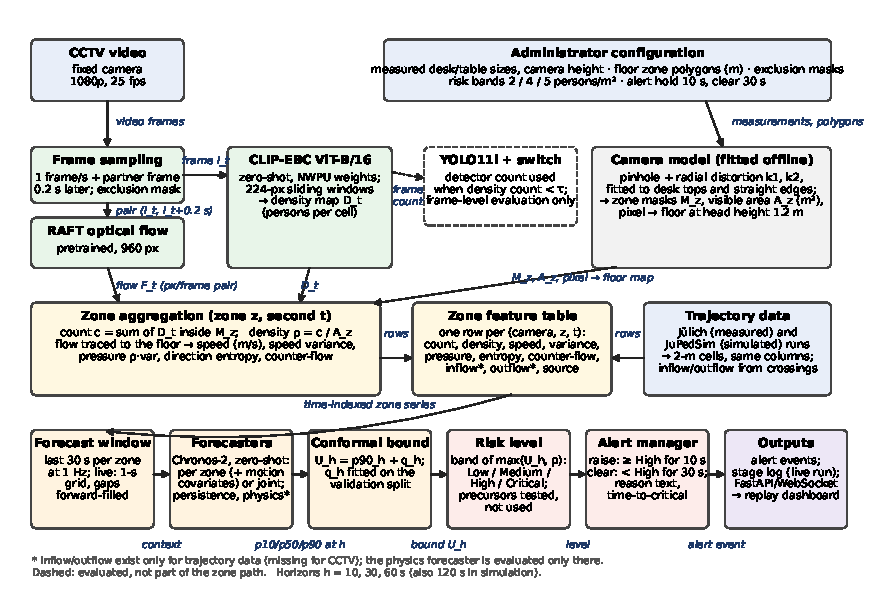
\includegraphics[width=\textwidth]{pipeline.pdf}
\CSfigcap{CrowdSafe pipeline: solid blocks form the deployed path; the dashed detector block is evaluated for frame-level counting only.}{fig:pipeline}
\end{figure*}

\section{Proposed Methodology}
\label{sec:method}
CrowdSafe is a chain of steps that turns camera frames into alerts, and each step works on the output of the previous one, as shown in Fig.~\ref{fig:pipeline}. A camera model, fitted once, relates image pixels to the floor. Every second, a frame becomes a map of where people are, and a pair of frames becomes a field of how people move; both are collected per floor zone into densities in \pmsq{} and motion statistics, stored as one row per zone and second. Every 5\,s, the recent rows of each zone are forecast, the calibrated upper bound of the forecast becomes a risk level, and sustained high levels become alerts on a dashboard. Each step below is first described in general terms and then illustrated with the classroom, J\"ulich and simulation data.

\subsection{Camera Calibration}
Density in \pmsq{} requires knowing which floor area each part of the image shows. CrowdSafe fits a camera model, namely a pinhole camera with radial lens distortion ($k_1,k_2$), focal length, position and tilt, by robust least squares to a few objects of known size in a still frame and to straight edges, which must appear straight once the distortion is removed. A tape measure is the only extra resource. The fitted model carries any pixel to a point on the floor at a chosen height, which the zone and motion steps rely on.
In classrooms H705 and H706, desk tops of measured length (1.00\,m) serve as rectangles, with each desk position left free so that the row and column spacing remain independent checks, and door frames and the ceiling duct serve as straight edges. In the computer lab H103, monitors hide most desk tops, so long table edges at measured positions, vertical edges and the measured camera height are used instead.

\subsection{Zone Definition and Area Computation}
The floor is then divided into zones on a plan in metres, small enough that a dangerous pocket is not averaged away by an empty corner. The camera model projects each zone into the image at the height where heads appear, which gives the image region $M_z$ that belongs to zone $z$ and the floor area $A_z$ that the camera actually sees. These two quantities later turn a count of people into a density.
Each classroom uses 3$\times$3 seating blocks plus the front aisle (4--16\,m$^2$ each), projected at seated head height (1.2\,m); in H103, a glass partition that shows the neighbouring room is masked out.

\subsection{People Counting}
Every second, a video frame passes to a pretrained density model, CLIP-EBC ViT-B/16 with NWPU-Crowd weights, used without any training~\cite{ma2025clipebc,wang2021nwpu}. Applied in non-overlapping 224-pixel windows (45 windows for a zero-padded 1080p frame), the model returns a density map $D_t$ of 135$\times$240 cells, one per 8$\times$8 pixels, whose values are expected numbers of heads, so the map can be summed over any image region. Person detectors return boxes instead, so YOLO11l and a YOLO11 head detector trained on CrowdHuman serve as baselines~\cite{yolo11,shao2018crowdhuman}. Because detectors can be more accurate when only a few people are present, combinations of detector and density-model frame counts are also tested: a hard switch to the detector below a threshold $\tau$, a constant or 50/50 weighting, and a learned per-frame weight. These combinations act on whole-frame counts and are compared at frame level, while the zone pipeline continues with the density map.
In the recordings, one frame per second of every classroom and lab video passes through CLIP-EBC; the detectors and combinations run on the 160 hand-labelled frames to select the counting route, as reported in Section~\ref{sec:count}.

\subsection{Zone Density Estimation in Persons per \texorpdfstring{m$^2$}{m2}}
The density map from the counting step meets the zone regions and areas from the zone step. Summing the map inside a zone region gives the count $c_{z,t}=\sum D_t\odot M_z$, and dividing by the visible area gives the density $\rho_{z,t}=c_{z,t}/A_z$ in \pmsq. Zones with less than 2\,m$^2$ in view are skipped, because their density would be unstable. This per-second density is the quantity that the rest of the pipeline monitors.
For H705, this step produces ten densities every second, one for each seating block and the aisle.

\subsection{Crowd Motion Feature Extraction}
Density shows how full a zone is; motion shows how the crowd behaves. The same sampled frame and a second frame 0.2\,s later pass to pretrained RAFT-large optical flow at 544$\times$960 pixels with 12 refinement iterations, and the flow is averaged into the same 135$\times$240 cells as $D_t$~\cite{teed2020raft}. The camera model carries each displacement to the floor, turning pixel shifts into velocities in m/s, weighted by the density map so that empty floor contributes nothing. Per zone, this gives the mean speed, the velocity variance, crowd pressure $\rho\cdot\mathrm{var}$, the entropy of an 8-bin direction histogram and the share of counter-flow~\cite{helbing2007}. The number of people crossing a zone boundary per second (inflow and outflow) needs individual trajectories, so these values exist only where trajectories exist.
For the classroom recordings, all motion values come from RAFT and inflow and outflow remain empty; for J\"ulich and simulated runs, speeds and boundary crossings come directly from each trajectory.

\subsection{Zone Feature Table Construction}
All measurements meet in a single table with one row per camera (or run), zone and second, holding count, density, the motion values, inflow, outflow and the data source. Forecasting and alerting read only this table, so every source that fills the table is evaluated in exactly the same way.
The classroom CCTV fills the table through the density and motion steps. J\"ulich trajectories and JuPedSim simulations fill the table directly, with 2\,m$\times$2\,m floor cells as zones, and the J\"ulich densities agree exactly with PedPy on six checked runs~\cite{pedpy}. In this way, dangerous densities that the classrooms never reach pass through the same downstream steps.

\subsection{Crowd Density Forecasting}
Every 5\,s, the last 30\,s of each zone are read from the table as a regular 1-Hz series and forecast 10, 30 and 60\,s ahead. The forecaster is Chronos-2, a pretrained time-series model used zero-shot~\cite{ansari2025chronos2}. The model runs either \emph{per zone}, with pressure, inflow, outflow and mean speed as additional inputs (set to zero when missing), or \emph{jointly} over all zones of one camera so that neighbouring zones inform each other, and returns the 10, 50 and 90\,\% quantiles for each zone and horizon. Two simple forecasters serve as baselines: \emph{persistence}, which repeats the last value, and a \emph{physics} fill-rate model, $\rho+(q_{\mathrm{in}}-q_{\mathrm{out}})\,h/A_z$, which needs inflow and outflow. In live operation, a second skipped by a slow cycle is filled with the previous value so that the series stays regular. The horizon limits how early a warning can arrive, but the horizon is not the warning time itself.
Because most J\"ulich runs last only 1--3\,min, horizons of 10--60\,s apply there and on CCTV, with 120\,s added on the longer simulations; the physics model runs only on J\"ulich and simulated data.

\subsection{Reliable Upper Bound via Conformal Calibration}
The 90\,\% quantile of a forecaster carries no guarantee of being exceeded only 10\,\% of the time, and point forecasts have no spread at all. CrowdSafe therefore calibrates the upper bound with split conformal prediction~\cite{angelopoulos2023conformal}. On validation runs, the amount by which the realised density rose above the 90\,\% quantile is measured, and the finite-sample 90\,\% quantile of these residuals becomes an offset $q_h$ for each horizon. New forecasts then carry the bound $U_{z,h}=\max(0,\,\mathrm{p90}_{z,h}+q_h)$, the worst case on which the risk step operates.
The offsets are fitted on the validation cameras (cam01, cam03), 39 J\"ulich validation runs and four validation scenarios, and applied only to the test data. On CCTV, the Chronos-2 offsets are tiny (0.001--0.02\,\pmsq), while for persistence the offset of 0.14--0.18\,\pmsq{} forms the whole bound.

\subsection{Risk Classification (Low, Medium, High, Critical)}
The calibrated bounds over all horizons and the current density combine into a worst case, $W_z=\max(\max_h U_{z,h},\,\rho_z)$, mapped to Low ($<2$), Medium (2--4), High (4--5) or Critical ($\geq 5$\,\pmsq). The first horizon whose bound reaches 5\,\pmsq{} is reported as the time to critical. Before the first forecast of a run, only the current density is used.
On the H705 recording, for example, a zone at 1.6\,\pmsq{} appears as Medium because the forecast bound of that zone exceeds 2\,\pmsq, as visible in Fig.~\ref{fig:dashboard}.

\subsection{Precursor-Based Risk Escalation}
The motion values from the feature table can raise the level of a zone by one step when they signal trouble: high pressure, direction entropy or counter-flow, low speed, rising density with falling speed (flow collapse), or a fast rise in density. Each signal is kept only if, on validation data, the signal predicts that a zone at 2--4\,\pmsq{} will reach 4\,\pmsq{} within 60\,s at least twice as often as chance.
The thresholds are tuned on the pooled J\"ulich and simulation validation runs; no signal passes, as detailed in Section~\ref{sec:negative}, so the final system raises levels from the forecast bound alone.

\subsection{Alert Generation}
Levels change every 5\,s and can flicker, so an alert manager adds hysteresis: an alert is raised when a zone stays High or above for 10\,s and cleared once the zone has stayed below High for 30\,s. Each alert records the zone, the highest level reached, the time to critical and a short reason, such as ``forecast upper bound 4.2 \pmsq{} (now 1.8)''.
In the held-out J\"ulich corridor run shown in Fig.~\ref{fig:timeline}, the bound of zone c3\_2 crosses 4\,\pmsq{} and an alert is raised at 219\,s, 49\,s before the zone itself reaches 4\,\pmsq.

\subsection{Dashboard Visualisation}
Finally, the zones, levels, forecasts and alerts are presented to an operator. A FastAPI/WebSocket server replays a stored run by re-running the risk and alert steps on the feature rows and forecasts of the run, and streams one message per second to a Next.js dashboard: the camera video with zones coloured by level and labelled with density, the forecast of a selected zone and the alert feed. The live pipeline described in Section~\ref{sec:runtime} runs the same steps directly on a camera stream.
Fig.~\ref{fig:dashboard} shows the dashboard replaying the H705 recording.

\begin{figure}[!t]
\centering
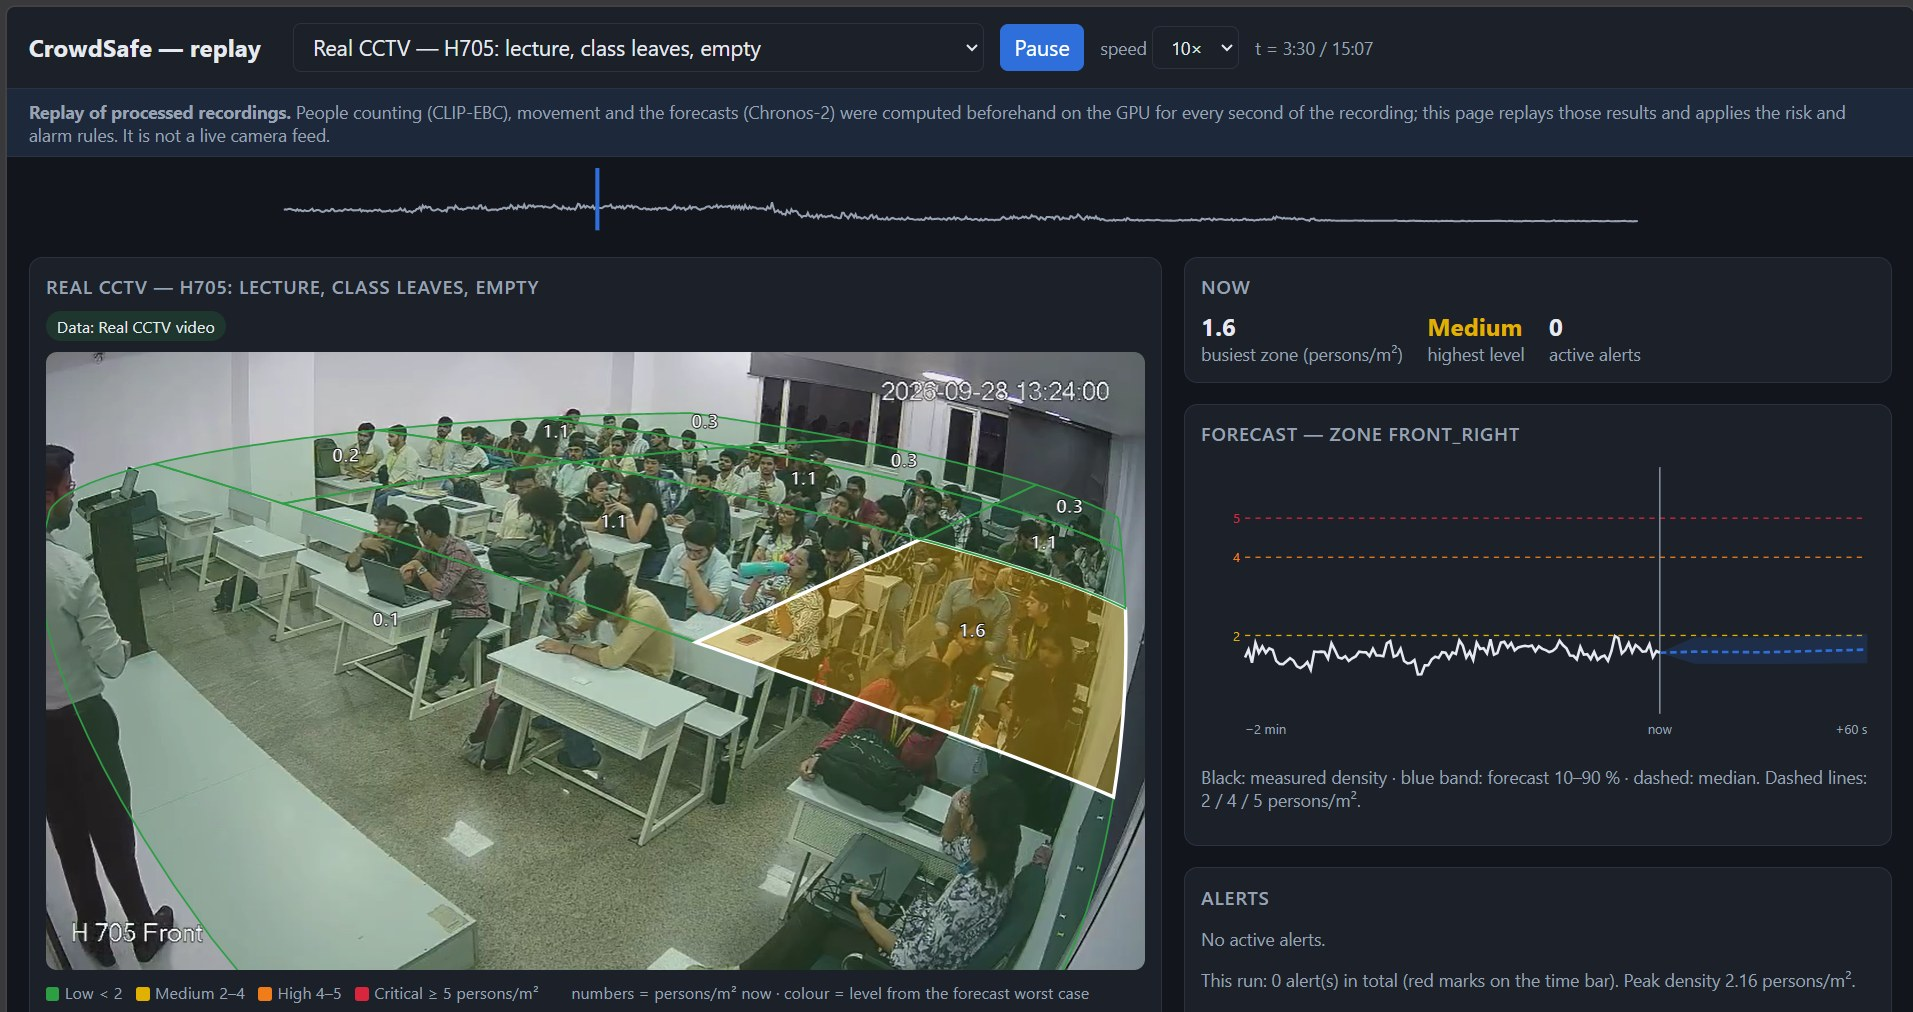
\includegraphics[width=\columnwidth]{dashboard.jpg}
\CSfigcap{Replay dashboard on the H705 recording.}{fig:dashboard}
\end{figure}

\section{Datasets and Experimental Setup}
Table~\ref{tab:data} lists the four data sources, the split of each and the role of each in the evaluation.

\begin{table}[!t]
\CStabcap{Datasets and Their Role}{tab:data}
\centering
\scriptsize
\setlength{\tabcolsep}{3pt}
\begin{tabular}{@{}p{1.35cm}p{3.75cm}p{2.7cm}@{}}
\toprule
Dataset & Content and split & Use \\
\midrule
Own CCTV & 4 cameras, 3 rooms, 2.6\,h; 160 labelled frames, 6,715 heads; val cam01/03, test cam02/04 & counting, zone density, forecasting, latency \\
ShanghaiTech A/B~\cite{zhang2016mcnn} & test sets, 182 / 316 images & counting check \\
J\"ulich~\cite{julich_archive} & val 39 runs; test: corridor 2013~\cite{julich_uni2013} (9 runs), entrance~\cite{julich_semicircle} (1) & real dense crowds \\
JuPedSim~\cite{jupedsim} & 16 scenarios; val 4, test 5 & dangerous events (to 8\,\pmsq) \\
\bottomrule
\end{tabular}
\end{table}

\subsection{Own CCTV Recordings and Annotation}
Two views of classroom H705, classroom H706 and computer lab H103 are recorded with permission (2.6\,h, 1080p). Head points on 160 frames are annotated by correcting model pre-labels. The busiest zone reaches 3.2\,\pmsq, so the recordings contain no dangerous density. No faces or identities are stored.

\subsection{ShanghaiTech Benchmark}
ShanghaiTech A and B are standard counting benchmarks, and only the test sets serve here to check the zero-shot models~\cite{zhang2016mcnn,li2018csrnet}.

\subsection{J\"ulich Pedestrian Experiments}
The first test experiment is a unidirectional corridor, previously analysed for fundamental diagrams~\cite{julich_uni2013,cao2017fundamental}. The second is an entrance crowd, previously studied for collective crowd behaviour~\cite{julich_semicircle,sieben2017collective}. The two experiments reach 5.3 and 9.0\,\pmsq.

\subsection{JuPedSim Simulated Scenarios}
Sixteen scenarios in four layouts (classroom, corridor bottleneck, two-exit hall, bidirectional corridor) include arrival surges and exit closures. Desired walking speeds follow $\mathcal{N}(1.34, 0.26^2)$\,m/s~\cite{weidmann1993}. Simulations follow model rules, not real behaviour.

\subsection{Train, Validation, and Test Splits}
No model is trained. Fusion parameters are fitted leave-one-room-out. Conformal offsets use validation cameras, experiments or scenarios and are applied to disjoint test ones, and precursor thresholds use the pooled J\"ulich and simulation validation splits. Test data serve no fitting.

\subsection{Evaluation Metrics}
Counting uses the mean absolute error (MAE) in people per frame, and zone density the MAE in \pmsq. Forecasts use the MAE and the \emph{coverage}, the share of test forecasts at or below the bound (target 0.90). For alerts, an \emph{event} is the first second at which a zone reaches 4 (or 5)\,\pmsq{} after monitoring starts. An event counts as \emph{warned in time} if an alert is raised at most (longest horizon + 10\,s) before the event and more than 15\,s after monitoring begins. Lead time is the time from alert to event, and a \emph{false alarm} is an alert with no event within 120\,s, counted per zone-hour.

\subsection{Hardware and Software}
Density maps, flow, Chronos-2 and latency run on one shared NVIDIA A100 (40\,GB); label-based counting uses ONNX models on a CPU. Simulations use JuPedSim 1.4.2 and analysis uses PedPy 1.5.1. No model is trained; the deployed path has about 222\,M parameters, feature extraction for all 2.6\,h of CCTV takes 33.5\,min on the A100, and the 16 simulations take 9.7\,min on a CPU.

\section{Results and Discussion}

\subsection{Counting Accuracy on ShanghaiTech}
\label{sec:sha}
Table~\ref{tab:counting} compares the counting models. Zero-shot CLIP-EBC reaches an MAE of 66.95 on part A and 11.66 on part B, close to CSRNet trained on ShanghaiTech, while detectors miss most people in these dense images.

\begin{table}[!t]
\CStabcap{Counting MAE (People per Frame)}{tab:counting}
\centering
\scriptsize
\setlength{\tabcolsep}{3pt}
\begin{tabular}{@{}lcccc@{}}
\toprule
Model & H705 & H706 & H103 & ShanghaiTech A / B \\
\midrule
CLIP-EBC (zero-shot) & \textbf{5.10} & \textbf{2.58} & \textbf{1.97} & 66.95 / 11.66 \\
YOLO11l & 6.36 & 6.53 & 17.63 & 418.3 / 92.8 \\
CrowdHuman heads & 8.04 & 6.23 & 28.23 & 374.2 / 70.2 \\
MCNN$^\dagger$~\cite{zhang2016mcnn} & -- & -- & -- & 110.2 / 26.4 \\
CSRNet$^\dagger$~\cite{li2018csrnet} & -- & -- & -- & 68.2 / 10.6 \\
\bottomrule
\multicolumn{5}{@{}l}{\scriptsize $^\dagger$Published results, trained on ShanghaiTech. Frames: 100 / 30 / 30.}
\end{tabular}
\end{table}

\subsection{Counting Accuracy on CCTV and Fusion Ablation}
\label{sec:count}
On the classroom CCTV, CLIP-EBC is the most accurate model in every room (Table~\ref{tab:counting}). Detectors undercount by 6--17 people per frame because desks, students and monitors hide bodies, and detectors are better only in near-empty frames (below 20 people in H705: 0.86 against 1.15). Within one room, fusion appears strong (constant weight 1.59, learned weight 2.09, CLIP-EBC 5.30), but the leave-one-room-out evaluation in Table~\ref{tab:fusion} reverses this ranking.

\begin{table}[!t]
\CStabcap{Leave-One-Room-Out Counting MAE}{tab:fusion}
\centering
\scriptsize
\begin{tabular}{@{}lcccc@{}}
\toprule
Method & H705 & H706 & H103 & Mean \\
\midrule
Hard switch & 5.08 & 2.51 & 1.89 & \textbf{3.16} \\
CLIP-EBC alone & 5.10 & 2.58 & 1.97 & 3.22 \\
50/50 average & 1.68 & 3.45 & 8.31 & 4.48 \\
Constant weight & 4.17 & 2.72 & 6.79 & 4.56 \\
Learned fusion & 4.30 & 3.08 & 8.29 & 5.22 \\
YOLO11l alone & 6.36 & 6.53 & 17.63 & 10.17 \\
\bottomrule
\end{tabular}
\end{table}

\subsection{Calibration Accuracy}
Reprojection errors are 3.6--4.2\,px. On distances excluded from the fit, the H705 row spacing measures 0.99 against 0.96\,m (+3\,\%) and the mean desk spacing differs by $-5$\,\%; an H706 door measures 1.23 against 1.12\,m (+10\,\%); and lab table edges lie within 0.03--0.18\,m. The calibration is therefore treated as accurate to about $\pm 5$\,\%.

\subsection{Zone Density Accuracy}
Zone-density MAE is 0.101 (H705), 0.081 (H706) and 0.078\,\pmsq{} (H103), with 94--98\,\% of heads inside a zone, and changing the head height from 1.1 to 1.6\,m alters the MAE by at most 0.03. These errors are small next to the 2\,\pmsq{} band width, although the measurements extend only up to 1.67\,\pmsq.

\subsection{Forecasting Accuracy and Upper-Bound Reliability}
\label{sec:forecast}
Table~\ref{tab:forecast} reports forecasting results on the test splits. Chronos-2 matches persistence on average error, and the calibrated Chronos-2 bound holds near 90\,\% on all sources, while persistence drops to 0.66 on J\"ulich at 30\,s. Where the true density is at least 4\,\pmsq, every bound under-covers, but Chronos-2 keeps 0.76--0.88 on J\"ulich against 0.56--0.78 for persistence. The CCTV test cameras never reach 2\,\pmsq.

\begin{table}[!t]
\CStabcap{Forecasting on Test Splits (Ranges over Horizons)}{tab:forecast}
\centering
\scriptsize
\setlength{\tabcolsep}{2.5pt}
\begin{tabular}{@{}llccc@{}}
\toprule
Data & Model & MAE (\pmsq) & Coverage & Cov., $\rho\geq 4$ \\
\midrule
CCTV & Chronos-2 joint & .064--.097 & .89--.91 & -- \\
 & Persistence & .074--.105 & .91--.93 & -- \\
J\"ulich & Chronos-2 per zone & .38--.73 & .88--.93 & .76--.88 \\
 & Persistence & .39--.71 & .66--.85 & .56--.78 \\
Simulation & Chronos-2 joint & .16--.76 & .91--.96 & .77--.84 \\
 & Persistence & .17--.75 & .87--.93 & .62--.71 \\
\bottomrule
\multicolumn{5}{@{}l}{\scriptsize Horizons 10--60\,s (simulation 10--120\,s). Target coverage 0.90.}
\end{tabular}
\end{table}

\subsection{Early-Warning Performance}
Table~\ref{tab:alerts} reports the alert results. Alerts on current density never warn before a zone reaches 4\,\pmsq. Forecast-driven alerts warn in time for about a third of the 47 simulated events, with median leads of 7.5\,s (Chronos-2) and 25\,s (physics, with more false alarms), and for one of nine J\"ulich events. Fig.~\ref{fig:timeline} shows the J\"ulich run with the Chronos-2 success: zone c3\_2 is warned 49\,s ahead, while earlier alerts in other zones fall outside the protocol window. For a 5\,\pmsq{} event, an alert at 4\,\pmsq{} is itself an early warning, and current-density alerts warn for 38\,\% of 34 simulated events. The classroom CCTV produces no events and no false alarms in 8.6 zone-hours. Zones fill from safe to 4\,\pmsq{} in about 10--20\,s, which explains the short leads: the forecast horizon is not the warning time.

\begin{table}[!t]
\CStabcap{Events Warned in Time (Median Lead; False Alarms per Zone-Hour)}{tab:alerts}
\centering
\scriptsize
\setlength{\tabcolsep}{2.5pt}
\begin{tabular}{@{}lccc@{}}
\toprule
Alert driver & Sim., 4\,\pmsq & J\"ulich, 4\,\pmsq & Sim., 5\,\pmsq \\
 & 47 events & 9 events & 34 events \\
\midrule
Current density & 0\,\% & 0/9 & 38\,\% (5\,s; 0.6) \\
Persistence & 0\,\% & 1/9 (4\,s; 0) & 38\,\% (10\,s; 0.7) \\
Physics & 32\,\% (25\,s; 2.1) & 1/9 (59\,s; 11.9) & 23.5\,\% (47.5\,s; 3.2) \\
Chronos-2 per zone & 34\,\% (7.5\,s; 1.6) & 1/9 (49\,s; 1.8) & 26.5\,\% (35\,s; 2.8) \\
Chronos-2 joint & 30\,\% (7.5\,s; 1.5) & 1/9 (18\,s; 0.5) & 26.5\,\% (25\,s; 2.7) \\
\bottomrule
\end{tabular}
\end{table}

\begin{figure}[!t]
\centering
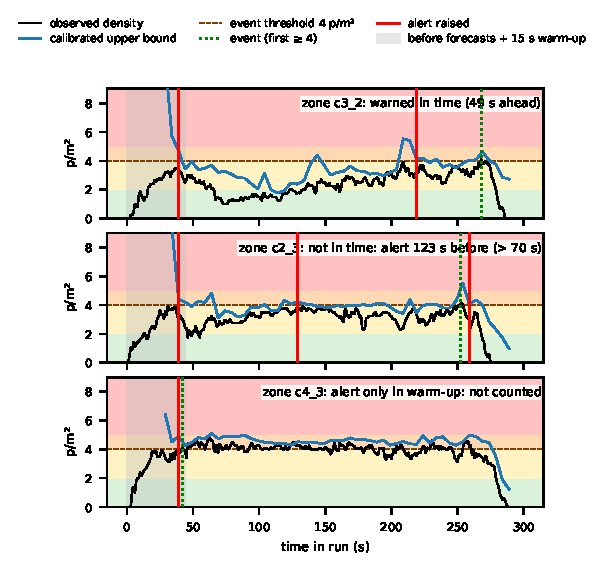
\includegraphics[width=\columnwidth]{alert_timeline.pdf}
\CSfigcap{Alert timeline of a held-out J\"ulich corridor run (Chronos-2 per zone).}{fig:timeline}
\end{figure}

\subsection{Runtime Performance}
\label{sec:runtime}
On one shared A100 with cam02 played at real speed, the live pipeline has a median latency of 0.49\,s (p95 1.6\,s) from frame to alert state, with 94\,\% of 1-s cycles on time and 2.0\,GB of GPU memory; median stage times are 159\,ms (CLIP-EBC), 103\,ms (RAFT) and 54\,ms (Chronos-2, every 5\,s). Unpaced, 908\,s of video take 196\,s (4.6$\times$ real time). A laptop CPU needs about 19\,s per second of video. Table~\ref{tab:models} lists the size, input, output and time of each model.

\begin{table}[!t]
\CStabcap{Models: Size, Data Passed and Time per Call}{tab:models}
\centering
\scriptsize
\setlength{\tabcolsep}{2.5pt}
\begin{tabular}{@{}p{1.5cm}p{0.85cm}p{1.9cm}p{1.95cm}p{1.3cm}@{}}
\toprule
Model & Params & Input & Output & A100 time \\
\midrule
CLIP-EBC ViT-B/16 & $\approx$97\,M & 45 windows of 224$\times$224 & density map, 135$\times$240 & 159\,ms \\
RAFT-large & $\approx$5.3\,M & 2 frames, 544$\times$960 & flow, 135$\times$240 cells & 103\,ms \\
Chronos-2 & 120\,M & last 30\,s per zone & 3 quantiles $\times$ 3 horizons & 54\,ms per 5\,s \\
YOLO11l (baseline) & $\approx$25\,M & frame at 1280\,px & person boxes & 15.5\,ms \\
\bottomrule
\multicolumn{5}{@{}p{7.6cm}@{}}{$\approx$: estimated from the fp32 model file size; Chronos-2 from the model card. Times: live medians (YOLO11l: single benchmark).}
\end{tabular}
\end{table}

\subsection{Comparison with Existing Systems}
On ShanghaiTech A, zero-shot CLIP-EBC is close to CSRNet and better than MCNN, both trained on that dataset, as listed in Table~\ref{tab:counting}; the training regimes differ, so the comparison makes no claim of superiority. System-level studies use different data and metrics and admit no numerical comparison~\cite{cao2013video,niu2020overcrowdedness}.

\subsection{Negative Findings}
\label{sec:negative}
\emph{Learned fusion} appears best within one room only because detector and density errors cancel there; on unseen rooms, learned fusion is the worst combination (Table~\ref{tab:fusion}). \emph{Motion precursors:} on J\"ulich validation alone, slowing (precision 0.54, 3.8$\times$ the base rate) and direction entropy (2.0$\times$) pass, but pooled with simulation none passes, so none is used. Variants of alert timing (shorter hold, rate of rise, shorter history) each help one forecaster and hurt another, so the default stays. A looser early scoring, which credited alerts raised at the start of monitoring, reported 56\,\% and 86\,\% warned; only the strict values are reported here.

The evaluation has bounded scope. Calibration is approximate and assumes seated head height. The classroom CCTV contains no dangerous densities, so danger-level results rest on nine real J\"ulich events and on simulation. CCTV speeds lack validation against ground truth, and inflow and outflow are not measured from CCTV. Latency is measured for one camera on a shared GPU.

\section{Conclusion and Future Work}

\subsection{Conclusion}
CrowdSafe addresses the problem of measuring and anticipating dangerous local crowd density from CCTV cameras that are already installed, without calibration data or model training. The measurement part of this problem is solved to a satisfactory level: pretrained, zero-shot components turn existing CCTV into zone density with errors around 0.1\,\pmsq{} and run live on one GPU in under a second. The forecasting part is also addressed reliably: a conformally calibrated zero-shot forecaster provides an upper bound that holds near the 90\,\% target and degrades less than persistence at high density. Early warning is achieved partially: forecast-driven alerts warn for about a third of simulated dangerous events and for one of nine real events, seconds rather than minutes ahead.

\subsection{Future Work}
Longer warnings need information beyond a single view: entrance cameras, gate counters, schedules and inflow measured across zone boundaries from CCTV. Further steps are validating CCTV speeds, recording staged crowding with a calibrated camera, density-conditional calibration and multi-camera latency tests.

\begin{thebibliography}{23}
\bibitem{fruin1971} J.~J. Fruin, \emph{Pedestrian Planning and Design}. New York, NY, USA: Metropolitan Association of Urban Designers and Environmental Planners, 1971.
\bibitem{helbing2007} D.~Helbing, A.~Johansson, and H.~Z. Al-Abideen, ``Dynamics of crowd disasters: An empirical study,'' \emph{Phys. Rev. E}, vol.~75, no.~4, p.~046109, 2007, doi: 10.1103/PhysRevE.75.046109.
\bibitem{zhang2016mcnn} Y.~Zhang, D.~Zhou, S.~Chen, S.~Gao, and Y.~Ma, ``Single-image crowd counting via multi-column convolutional neural network,'' in \emph{Proc. IEEE Conf. Comput. Vis. Pattern Recognit. (CVPR)}, 2016, pp. 589--597.
\bibitem{li2018csrnet} Y.~Li, X.~Zhang, and D.~Chen, ``CSRNet: Dilated convolutional neural networks for understanding the highly congested scenes,'' in \emph{Proc. IEEE Conf. Comput. Vis. Pattern Recognit. (CVPR)}, 2018, pp. 1091--1100, doi: 10.1109/CVPR.2018.00120.
\bibitem{ma2025clipebc} Y.~Ma, V.~Sanchez, and T.~Guha, ``CLIP-EBC: CLIP can count accurately through enhanced blockwise classification,'' in \emph{Proc. IEEE Int. Conf. Multimedia Expo (ICME)}, 2025, arXiv:2403.09281.
\bibitem{wang2021nwpu} Q.~Wang, J.~Gao, W.~Lin, and X.~Li, ``NWPU-Crowd: A large-scale benchmark for crowd counting and localization,'' \emph{IEEE Trans. Pattern Anal. Mach. Intell.}, vol.~43, no.~6, pp. 2141--2149, 2021, doi: 10.1109/TPAMI.2020.3013269.
\bibitem{yolo11} G.~Jocher and J.~Qiu, ``Ultralytics YOLO11,'' version 11.0.0, 2024. [Online]. Available: \url{https://github.com/ultralytics/ultralytics}
\bibitem{shao2018crowdhuman} S.~Shao, Z.~Zhao, B.~Li, T.~Xiao, G.~Yu, X.~Zhang, and J.~Sun, ``CrowdHuman: A benchmark for detecting human in a crowd,'' arXiv:1805.00123, 2018.
\bibitem{julich_archive} Forschungszentrum J\"ulich, ``Data archive of experimental data from studies about pedestrian dynamics.'' [Online]. Available: \url{https://ped.fz-juelich.de/da/} (accessed Oct. 2026).
\bibitem{pedpy} T.~Schr\"odter and The PedPy Development Team, ``PedPy: Pedestrian dynamics analysis library,'' version 1.5.1, Zenodo, doi: 10.5281/zenodo.21476844.
\bibitem{jupedsim} The JuPedSim Development Team, ``JuPedSim: Simulating pedestrian dynamics,'' version 1.4.2. [Online]. Available: \url{https://www.jupedsim.org}
\bibitem{zhang2017stresnet} J.~Zhang, Y.~Zheng, and D.~Qi, ``Deep spatio-temporal residual networks for citywide crowd flows prediction,'' in \emph{Proc. AAAI Conf. Artif. Intell.}, vol.~31, no.~1, 2017, doi: 10.1609/aaai.v31i1.10735.
\bibitem{niu2020overcrowdedness} Y.~Niu, W.~Shi, W.~Liu, S.~He, J.~Pan, and A.~B. Chan, ``Over-crowdedness alert! Forecasting the future crowd distribution,'' arXiv:2006.05127, 2020.
\bibitem{ansari2024chronos} A.~F. Ansari \emph{et al.}, ``Chronos: Learning the language of time series,'' \emph{Trans. Mach. Learn. Res.}, 2024.
\bibitem{ansari2025chronos2} A.~F. Ansari \emph{et al.}, ``Chronos-2: From univariate to universal forecasting,'' arXiv:2510.15821, 2025.
\bibitem{angelopoulos2023conformal} A.~N. Angelopoulos and S.~Bates, ``Conformal prediction: A gentle introduction,'' \emph{Found. Trends Mach. Learn.}, vol.~16, no.~4, pp. 494--591, 2023, doi: 10.1561/2200000101.
\bibitem{cao2013video} L.~Cao and K.~Huang, ``Video-based crowd density estimation and prediction system for wide-area surveillance,'' \emph{China Commun.}, vol.~10, no.~5, pp. 79--88, 2013, doi: 10.1109/CC.2013.6520940.
\bibitem{teed2020raft} Z.~Teed and J.~Deng, ``RAFT: Recurrent all-pairs field transforms for optical flow,'' in \emph{Proc. Eur. Conf. Comput. Vis. (ECCV)}, 2020, pp. 402--419.
\bibitem{julich_uni2013} Forschungszentrum J\"ulich, ``Pedestrian flow in a unidirectional corridor (BaSiGo project),'' Pedestrian Dynamics Data Archive, 2013, doi: 10.34735/ped.2013.6.
\bibitem{julich_semicircle} Forschungszentrum J\"ulich, ``Entrance 1, entry without guiding barriers (semicircle setup),'' Pedestrian Dynamics Data Archive, 2013, doi: 10.34735/ped.2013.2.
\bibitem{cao2017fundamental} S.~Cao, A.~Seyfried, J.~Zhang, S.~Holl, and W.~Song, ``Fundamental diagrams for multidirectional pedestrian flows,'' \emph{J. Stat. Mech.: Theory Exp.}, 2017, doi: 10.1088/1742-5468/aa620d.
\bibitem{sieben2017collective} A.~Sieben, J.~Schumann, and A.~Seyfried, ``Collective phenomena in crowds---Where pedestrian dynamics need social psychology,'' \emph{PLOS ONE}, vol.~12, no.~6, 2017, doi: 10.1371/journal.pone.0177328.
\bibitem{weidmann1993} U.~Weidmann, ``Transporttechnik der Fussg\"anger,'' Schriftenreihe des IVT, no.~90, ETH Z\"urich, Z\"urich, Switzerland, 1993.
\end{thebibliography}

\end{document}
